\documentclass[12pt]{article}

\usepackage{graphics}
\usepackage{epsfig}
\usepackage{times}
\usepackage{amsmath}
\usepackage{booktabs} % For formal tables
\usepackage{subcaption}
\usepackage{algorithm2e}
\usepackage{algorithmicx}
\usepackage[noend]{algpseudocode}
\usepackage{multirow}

\bibliographystyle{IEEEtran}

\graphicspath{ {Extras/images/} }

%Optional Package to add PDF bookmarks and hypertext links
\usepackage[pdftex,hypertexnames=false,linktocpage=true]{hyperref} 
\hypersetup{colorlinks=true,linkcolor=blue,anchorcolor=blue,citecolor=blue,filecolor=blue,urlcolor=blue,bookmarksnumbered=true,pdfview=FitB}

% The standard departmental thesis proposal format is the following:
%        30 pages
%        12 point type
%        1 inch margins all around = 6.5   inch column
%        (Total:  30 * 6.5   = 195 page-inches)
%
% For letter-size paper: 8.5 in x 11 in
% Latex Origin is 1''/1'', so measurements are relative to this.

\topmargin      0.0in
\headheight     0.0in
\headsep        0.0in
\oddsidemargin  0.0in
\evensidemargin 0.0in
\textheight     9.0in
\textwidth      6.5in
\linespread{1.5}


\newcommand{\todo}[1]{\textcolor{magenta}{{\sf (TODO: #1)}}}

%%%%%%%%%%%%%%%%%%%%%%%%
%responsible for making a glossary of terms
\usepackage[acronym,nonumberlist]{glossaries}
\makenoidxglossaries % use TeX to sort

%list of acryonms
\newacronym{ai}{AI}{Allen Iverson}

%%%%%%%%%%%%%%%%%%%%%%%%%

\begin{document}
\pagestyle{plain}
\pagenumbering{roman}
\title{{\bf Doctoral Thesis Proposal} \\
	\it Thesis proposal}
\author{ {\bf Allen Iverson}  \\
	Department of Electrical and Computer Engineering  \\
	Iowa State University\\
	{\small allen.iverson@iastate.edu}
}
\date{\today}

\maketitle
\pagebreak

\begin{abstract}
	The thesis proposal is a type of contract between the faculty and the student. 
	An accepted thesis proposal indicates that the work proposed by the student, 
	once completed, will be accepted by the faculty as sufficiently innovative and 
	substantial as to be recognized with the award of the degree. It is part of 
	the training of the student's research apprenticeship that the form of this 
	proposal must be as concise as those proposals required by major funding 
	agencies.
\end{abstract}

\pagebreak

\tableofcontents
\pagebreak
\cleardoublepage
\pagenumbering{arabic}

% Chapter 1
\section{Introduction}
\label{ch:intro}
This part provides an overall introduction of your work.

This section should talk about
\begin{enumerate}
	\item background
	\item problem statement
	\item motivation
	\item aims
\end{enumerate}
% Chapter 2: Lit Review
\section{Related work}\label{relatedworks}
This part talks about related work of your proposal.
 \gls{ai} attacks \cite{aiLow}
% Chapter 3
\section{Proposal Phase I}\label{proposal:p1}
talk about research questions and hypothesis this phase supports

\subsection{Summary}

% Chapter 4
\section{Proposal Phase II}\label{proposal:p2}
talk about research questions and hypothesis this phase supports

\subsection{Summary}
% Chapter 5
\section{Proposal Phase III} \label{proposal:p3}
talk about research questions and hypothesis this phase supports

\begin{figure}
	\centering
	\caption{Black Tops}
	\centering	
	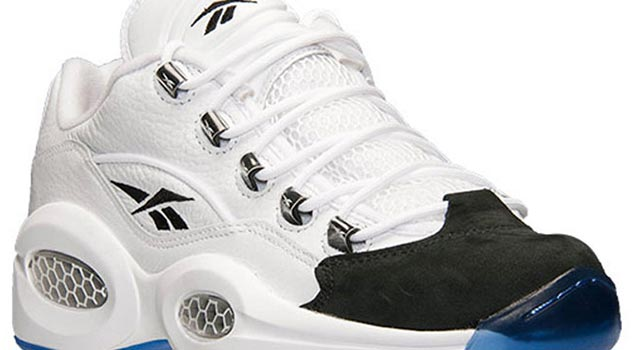
\includegraphics[scale=.6]{ai5.jpg}
	\label{tab:ai5}
\end{figure}

\subsection{Summary}
\section{Research Timeline}
\label{timeline}

Table \ref{tab:timeline} shows my plan for completion of the research.

\begin{table}[h]
	\begin{small}
		\begin{center}
			\begin{tabular}{lll}
				Due Date 		& Work 					& Progress\\
				\hline
				TBA 		& Preliminary results for magic & completed\\
				TBA 		& magic Analysis 	& in-progress\\
				TBA 	& magic Paper Writing & in-progress\\
				TBA 	& magic Submit Paper & not started\\
				TBA 	& Crossover Implementation & not started\\
				TBA 	& Crossover Testing/Analysis & not started\\
				TBA 	& Crossover Paper & not started\\
				TBA 	& Hall of Fame Testing & not started\\
				TBA 	& Hall of Fame  and Paper Writing & not started\\
				TBA  	& Thesis writing & not started\\
				TBA 		& Thesis defense & not started\\
			\end{tabular}
		\end{center}
	\end{small}
	\caption{Plan for completion of my research}
	\label{tab:timeline}
\end{table}

Thus, I plan to defend my thesis in TBA.

\pagebreak
% Chapter 7
\section{Conclusion} \label{conculsion}



\section{Acronyms}
\printnoidxglossaries
\pagebreak
\bibliography{mybib}


\end{document}